%==============================================================================
%  PAPER — artículo original RPMESP (asociación / implementación)
%  Compilar: bash compile.sh   ·   Anclas: ./tablas/   ·   SEED 20260710
%==============================================================================
% ---- Directivas de motor para editores independientes ---------------------
% !TEX program = latexmk
% !TEX TS-program = latexmk
% !BIB program = biber
% !BIB TS-program = biber
% (Overleaf/LaTeX-Workshop/TeXstudio/TeXShop: usan .latexmkrc de esta carpeta;
%  biblatex+biber requiere: pdflatex -> biber -> pdflatex -> pdflatex.)
%------------------------------------------------------------------------------
\documentclass[man,11pt,donotrepeattitle,floatsintext]{apa7}

% es-tabla: usar "Tabla" (RPMESP) en vez del "Cuadro" por defecto de babel-spanish.
\usepackage[english,spanish,es-noindentfirst,es-tabla]{babel}
% babel-spanish inserta un espacio fino antes de "%" por defecto (tipografía
% española tradicional); el estándar RPMESP de este paper pide "%" pegado.
\spanishplainpercent
% apa7 usa "Palabras Claves" (mayúscula, plural) para es; RPMESP pide "Palabras clave".
% Se aplica en \AtBeginDocument porque apa7 fija \keywordname ahí mismo (config/APA7spanish.txt)
% y ejecuta en orden de registro, así que esta redefinición debe ir DESPUÉS de la suya.
\AtBeginDocument{\renewcommand{\keywordname}{Palabras clave}}
\usepackage[utf8]{inputenc}
\usepackage[T1]{fontenc}
\usepackage{graphicx}
\usepackage{booktabs}
\usepackage{array}
\usepackage{amsmath}
\usepackage{csquotes}
\usepackage{orcidlink}
% titlesec es incompatible con apa7 (redefine \subparagraph con argumento
% obligatorio, lo que hace fallar \ttl@extract). Se reproduce aquí el mismo
% formato que se buscaba (títulos en negrita, a la izquierda, sin numeración)
% con \@startsection, reutilizando los saltos tipográficos que define apa7.
\makeatletter
\renewcommand{\section}{\@startsection {section}{1}{\z@}%
    {\b@level@one@skip}{\e@level@one@skip}%
    {\normalfont\large\bfseries\raggedright}}
\renewcommand{\subsection}{\@startsection{subsection}{2}{\z@}%
    {\b@level@two@skip}{\e@level@two@skip}%
    {\normalfont\normalsize\bfseries\raggedright}}
\makeatother

% style=vancouver: RPMESP exige Vancouver/ICMJE, no el estilo autor-año de apa7.
% La numeración en el texto ya era correlativa por aparición (sorting=none); lo que
% cambia es la puntuación de la lista de referencias.
\usepackage[style=vancouver,sorting=none,sortcites=true,backend=biber,maxnames=6,minnames=6,giveninits=true,doi=true,isbn=false,url=true]{biblatex}
% Vancouver estricto separa todos los autores con coma (sin "y"/"and" antes del
% último). spanish.lbx fuerza su "smart and"; se anula redefiniendo el delimitador
% final de nombre local (biblatex manual §3.9.60) con nombre y coma final.
% Spanish.lbx inserta su "smart and" (" y ", " y e") vía el contador interno
% \value{smartand}; con smartand=0 el render pasa por biblatex.def y aplican los
% delimitadores declarados abajo → restaurantes Vancouver con coma final.
\setcounter{smartand}{0}
\DeclareDelimFormat{finalnamedelim}{\addcomma\space}
\DeclareDelimFormat[bibliography]{finalnamedelim:andothers}{\addcomma\space et\adddot\space al\adddot}
% Prefijos nobiliarios en minúscula (von Elm, no Von Elm) en estilo Vancouver/NLM
\renewcommand*{\mkbibnameprefix}[1]{\MakeLowercase{#1}}
\ExecuteBibliographyOptions{useprefix=true}
% Inicializar revistas con abreviatura oficial NLM (Vancouver usa ISO 4):
% las entradas del .bib llevan journaltitle abreviado; en bibtex-mode el campo es "journal".
\addbibresource{referencias.bib}
% Suprimir URL cuando existe DOI (RPMESP muestra URL solo si no hay DOI)
\DeclareSourcemap{
  \maps[datatype=bibtex]{
    \map{
      \step[fieldsource=doi,final]
      \step[fieldset=url,null]
    }
  }
}

\graphicspath{{figuras/}}

\title{Asociación entre consumo reportado de suplementos con hierro y anemia moderada o severa en niños que recibieron suplementos: ENDES 2024, Perú}
\shorttitle{Consumo de hierro y anemia}
\leftheader{Autor et al.}


\authorsnames[1,1,2,3]{Rolando Bruno Bernaola Muñoz, Jaime Enrique Lincovil Curivil, Niels Pacheco-Barrios, César Daniel Reinoso Reinoso}
\authorsaffiliations{
  {Universidad Nacional de Ingeniería, Lima, Perú},
  {Brigham and Women's Hospital, Boston, Massachusetts, Estados Unidos},
  {Escuela Superior Politécnica de Chimborazo (ESPOCH), Riobamba, Ecuador}
}
\authornote{
Rolando Bruno Bernaola Muñoz \orcidlink{0000-0001-7159-887X}, \href{mailto:rolando.bernaola.m@uni.pe}{rolando.bernaola.m@uni.pe}.\\
Jaime Enrique Lincovil Curivil \orcidlink{0000-0003-4633-4033}, \href{mailto:jlincovilc@uni.edu.pe}{jlincovilc@uni.edu.pe}.\\
Niels Pacheco-Barrios \orcidlink{0000-0001-5586-8251}, \href{mailto:niels.pacheco.b@gmail.com}{niels.pacheco.b@gmail.com}.\\
César Daniel Reinoso Reinoso \orcidlink{0000-0002-1233-517X}, \href{mailto:cesard.reinoso@espoch.edu.ec}{cesard.reinoso@espoch.edu.ec} (correo institucional, ESPOCH); \href{mailto:cesardanielrrch@gmail.com}{cesardanielrrch@gmail.com} (correo personal).\\[6pt]
Correspondencia: Jaime Enrique Lincovil Curivil, Universidad Nacional de Ingeniería, Av. Túpac Amaru 210, Rímac, Lima, Perú; jlincovilc@uni.edu.pe.
}


%------------------------------------------------------------------------------
\abstract{

\textbf{Objetivos.} Estimar la asociación entre el consumo reportado de suplementos con hierro y la prevalencia de anemia moderada o severa en niños de 6 a 59 meses que recibieron suplementos y no tenían diagnóstico previo de anemia reportado por la madre, según la ENDES 2024.

\textbf{Materiales y métodos.} Se analizaron 6\,703 niños que habían recibido suplementos y no tenían un diagnóstico previo de anemia reportado por la madre (2\,194 con consumo en los 7 días previos). Se estimó la asociación mediante ponderación por el inverso de la probabilidad de exposición, combinada con el peso de diseño de la encuesta, y se realizó la inferencia mediante bootstrap estratificado con 2\,000 réplicas. También se evaluaron el ajuste por departamento, el análisis sin filtro de diagnóstico previo y una definición alternativa de consumo en 12 meses.

\textbf{Resultados.} Las prevalencias ajustadas fueron 9{,}3\% entre consumidores y 12{,}1\% entre no consumidores: una diferencia de $-2{,}8$ puntos porcentuales (IC del 95\%: $[-4{,}5;\,-1{,}2]$). En el análisis sin filtro de diagnóstico previo, restringido a casos completos ($n=8\,800$), la diferencia cayó a $-0{,}9$ puntos e incluyó el nulo (IC del 95\%: $[-2{,}6;\,0{,}9]$). Con la definición alternativa de consumo en 12 meses, la estimación puntual cambió de signo ($+2{,}4$ puntos), pero el intervalo fue compatible con el nulo (IC del 95\%: $[-0{,}2;\,4{,}7]$). La diferencia media de hemoglobina fue pequeña y compatible con el nulo.

\textbf{Conclusiones.} El consumo reportado en los siete días previos se asoció con menor prevalencia de anemia moderada o severa, pero la magnitud fue modesta y se atenuó al ajustar por departamento. La asociación fue compatible con el nulo al ampliar la población, y la estimación puntual cambió de signo con otra definición de exposición; el intervalo de confianza correspondiente también fue compatible con el nulo. Por el diseño transversal y la sensibilidad a la población y a la ventana de exposición, estos resultados no se interpretan como evidencia de eficacia farmacológica ni de una relación causal.
}

\keywords{Anemia; Hierro; Suplementos dietéticos; Encuestas epidemiológicas; Perú}

% Formato RPMESP: sin numeración de secciones ni subsecciones
\setcounter{secnumdepth}{0}

\begin{document}
\maketitle

\vspace{1.0em}
\begin{center}
	\large\textbf{Association between reported consumption of iron-containing supplements and moderate or severe anemia among children who received supplements: ENDES 2024, Peru}
\end{center}
\vspace{0.6em}

\vspace{0.5em}
\begin{otherlanguage*}{english}
\noindent\textbf{Abstract.}

\textbf{Objectives.} To estimate the association between reported consumption of iron-containing supplements and the prevalence of moderate or severe anemia among children aged 6--59 months who received supplements and had no maternal report of prior anemia diagnosis, using ENDES 2024.

\textbf{Materials and methods.} We analyzed 6,703 children who had received supplements and had no maternal report of prior anemia diagnosis (2,194 with consumption in the previous 7 days). We estimated the association using inverse-probability-of-exposure weighting combined with the survey design weight, with inference from stratified bootstrap with 2,000 replicates. We also examined adjustment by department, analysis without the prior-diagnosis filter, and an alternative 12-month consumption definition.

\textbf{Results.} Adjusted prevalences were 9.3\% among consumers and 12.1\% among non-consumers: a difference of $-2.8$ percentage points (95\% CI: $-4.5$ to $-1.2$). In the analysis without the prior-diagnosis filter, restricted to complete cases ($n=8{,}800$), the difference dropped to $-0.9$ points and included the null (95\% CI: $-2.6$ to $0.9$). With the 12-month consumption definition, the point estimate changed sign ($+2.4$ points), but its confidence interval was compatible with the null (95\% CI: $-0.2$ to $4.7$). The mean hemoglobin difference was small and compatible with the null.

\textbf{Conclusions.} Seven-day reported consumption was associated with lower prevalence of moderate or severe anemia, but the magnitude was modest and attenuated after adjustment for department. The association was compatible with the null when the population was expanded; under the alternative 12-month exposure definition, the point estimate changed sign, and its confidence interval was compatible with the null. Because of the cross-sectional design and sensitivity to the population and exposure window, these findings should not be interpreted as evidence of pharmacological efficacy or a causal relationship.

\vspace{0.4em}
\noindent\textbf{Keywords.} Anemia; Iron; Dietary supplements; Health surveys; Peru.
\end{otherlanguage*}

\vspace{1.0em}
\begin{center}
	\fbox{\parbox{0.92\textwidth}{
			\setlength{\parskip}{0.3em}
			\noindent\textbf{Mensajes clave}\\[0.4em]
			\textbf{¿Por qué se realizó el estudio?} La cobertura de entrega no permite conocer si los suplementos fueron consumidos en el hogar.\\
			\textbf{¿Qué se encontró?} En receptores sin diagnóstico previo reportado, el consumo durante los siete días anteriores se asoció con una prevalencia 2{,}8 puntos porcentuales menor de anemia moderada o severa. La estimación se atenuó a 2{,}4 puntos con ajuste departamental, fue compatible con el nulo en el análisis sin filtro de diagnóstico (casos completos) y la definición alternativa de 12 meses arrojó una estimación puntual de signo opuesto, pero compatible con el nulo.\\
			\textbf{¿Qué implican los hallazgos?} Los resultados sugieren complementar la medición de entrega con consumo y hemoglobina, pero no demuestran causalidad ni eficacia farmacológica.
		}}
\end{center}
\vspace{0.8em}

%==============================================================================
\section{INTRODUCCIÓN}
%==============================================================================

La anemia infantil constituye un problema de salud pública en los países de ingresos bajos y medios, y el Perú presenta una carga importante: según la ENDES 2024, el 33{,}7\% de los niños de 6 a 59 meses presentaba anemia \parencite{chaparro2019,stevens2022,inei2025endes}. Durante esta etapa del desarrollo, la anemia se ha asociado con consecuencias adversas a largo plazo, incluido el deterioro cognitivo y mayor morbimortalidad \parencite{zavaleta2017}. Sin embargo, la evaluación del estado de hierro requiere indicadores específicos como la ferritina \parencite{who2011ferritin}, mientras que la medición de hemoglobina en contextos andinos demanda ajuste por altitud, debido a que la hipoxia puede modificar fisiológicamente sus valores y afectar la clasificación de la anemia \parencite{gonzales2019}.

El Ministerio de Salud del Perú distribuye suplementos con hierro en gotas, jarabe y polvos de micronutrientes a través del sistema de salud público \parencite{who2016iron,minsa2022}. La cobertura de entrega informa si el suplemento llegó al niño o a su cuidador, pero no permite establecer si fue consumido en el hogar ni cómo se relaciona con el estado hematológico observado \parencite{pasricha2013,munares2018}. Por ello, la entrega, el consumo reportado y la hemoglobina deben considerarse dimensiones distintas del funcionamiento programático. Examinar estas dimensiones por separado permite identificar qué información aporta cada indicador y evita interpretar la cobertura de entrega como una medida directa del consumo o de la respuesta hematológica \parencite{low2013}.

En los datos observacionales, los niños que reciben y reportan consumir suplementos pueden diferir de aquellos que no lo hacen en edad, riesgo hematológico, contacto con los servicios de salud y otras características relevantes \parencite{austin2011,cole2008}. En consecuencia, una comparación directa puede combinar diferencias preexistentes entre los grupos con la asociación observada entre el consumo reportado y la anemia. Aunque estudios previos han documentado la brecha entre la entrega y el consumo de suplementos \parencite{munares2018}, todavía es limitada la evidencia sobre la relación entre el consumo reportado y el estado hematológico en condiciones programáticas reales.

El objetivo de este estudio fue estimar la asociación entre el consumo reportado de suplementos con hierro durante los siete días previos y la prevalencia de anemia moderada o severa en niños de 6 a 59 meses que habían recibido suplementos, sin diagnóstico previo de anemia reportado por la madre, según la ENDES 2024. Asimismo, se examinó la estabilidad de esta asociación frente al ajuste por departamento, la ampliación de la población analizada y una definición alternativa de consumo en 12 meses. El análisis se circunscribe a la relación observada entre consumo reportado y estado hematológico, y no pretende estimar eficacia farmacológica ni establecer una relación causal \parencite{low2013,neuberger2016}.



%==============================================================================
\section{MATERIALES Y MÉTODOS}
%==============================================================================

\subsection{Diseño y población}

Se realizó un estudio observacional, transversal, de análisis secundario de los microdatos públicos de la ENDES 2024. La encuesta utiliza un diseño multietápico y estratificado, con representatividad nacional y departamental \parencite{inei2025endes}, basado en la metodología DHS \parencite{dhs2023}. En el módulo de salud infantil se registró la hemoglobina capilar, medida mediante HemoCue, de 14\,428 niños. Los valores de hemoglobina se ajustaron por altitud conforme al procedimiento documentado en la base analítica y a los protocolos de referencia del INEI, el MINSA y la OMS. El reporte del estudio siguió las recomendaciones de la guía STROBE para estudios observacionales \parencite{vonelm2007strobe}.

De ellos, se seleccionaron los 9\,079 que recibieron al menos una presentación de suplemento en los 12 meses previos. El análisis principal se restringió a los 6\,908 sin diagnóstico previo de anemia reportado por la madre: esta población representa el grupo programático de interés ---niños receptores aún no diagnosticados---, aunque la restricción introduce selección porque la ENDES no registra cuándo ocurrió el diagnóstico ni cuándo se consumió el suplemento. Tras excluir los casos con covariables incompletas, la muestra analítica quedó en 6\,703 niños (2\,194 con consumo reportado y 4\,509 sin consumo; Figura~\ref{fig:flujo}). El análisis sin esa restricción se reporta en Resultados.

\begin{figure}[htbp]
	\centering
	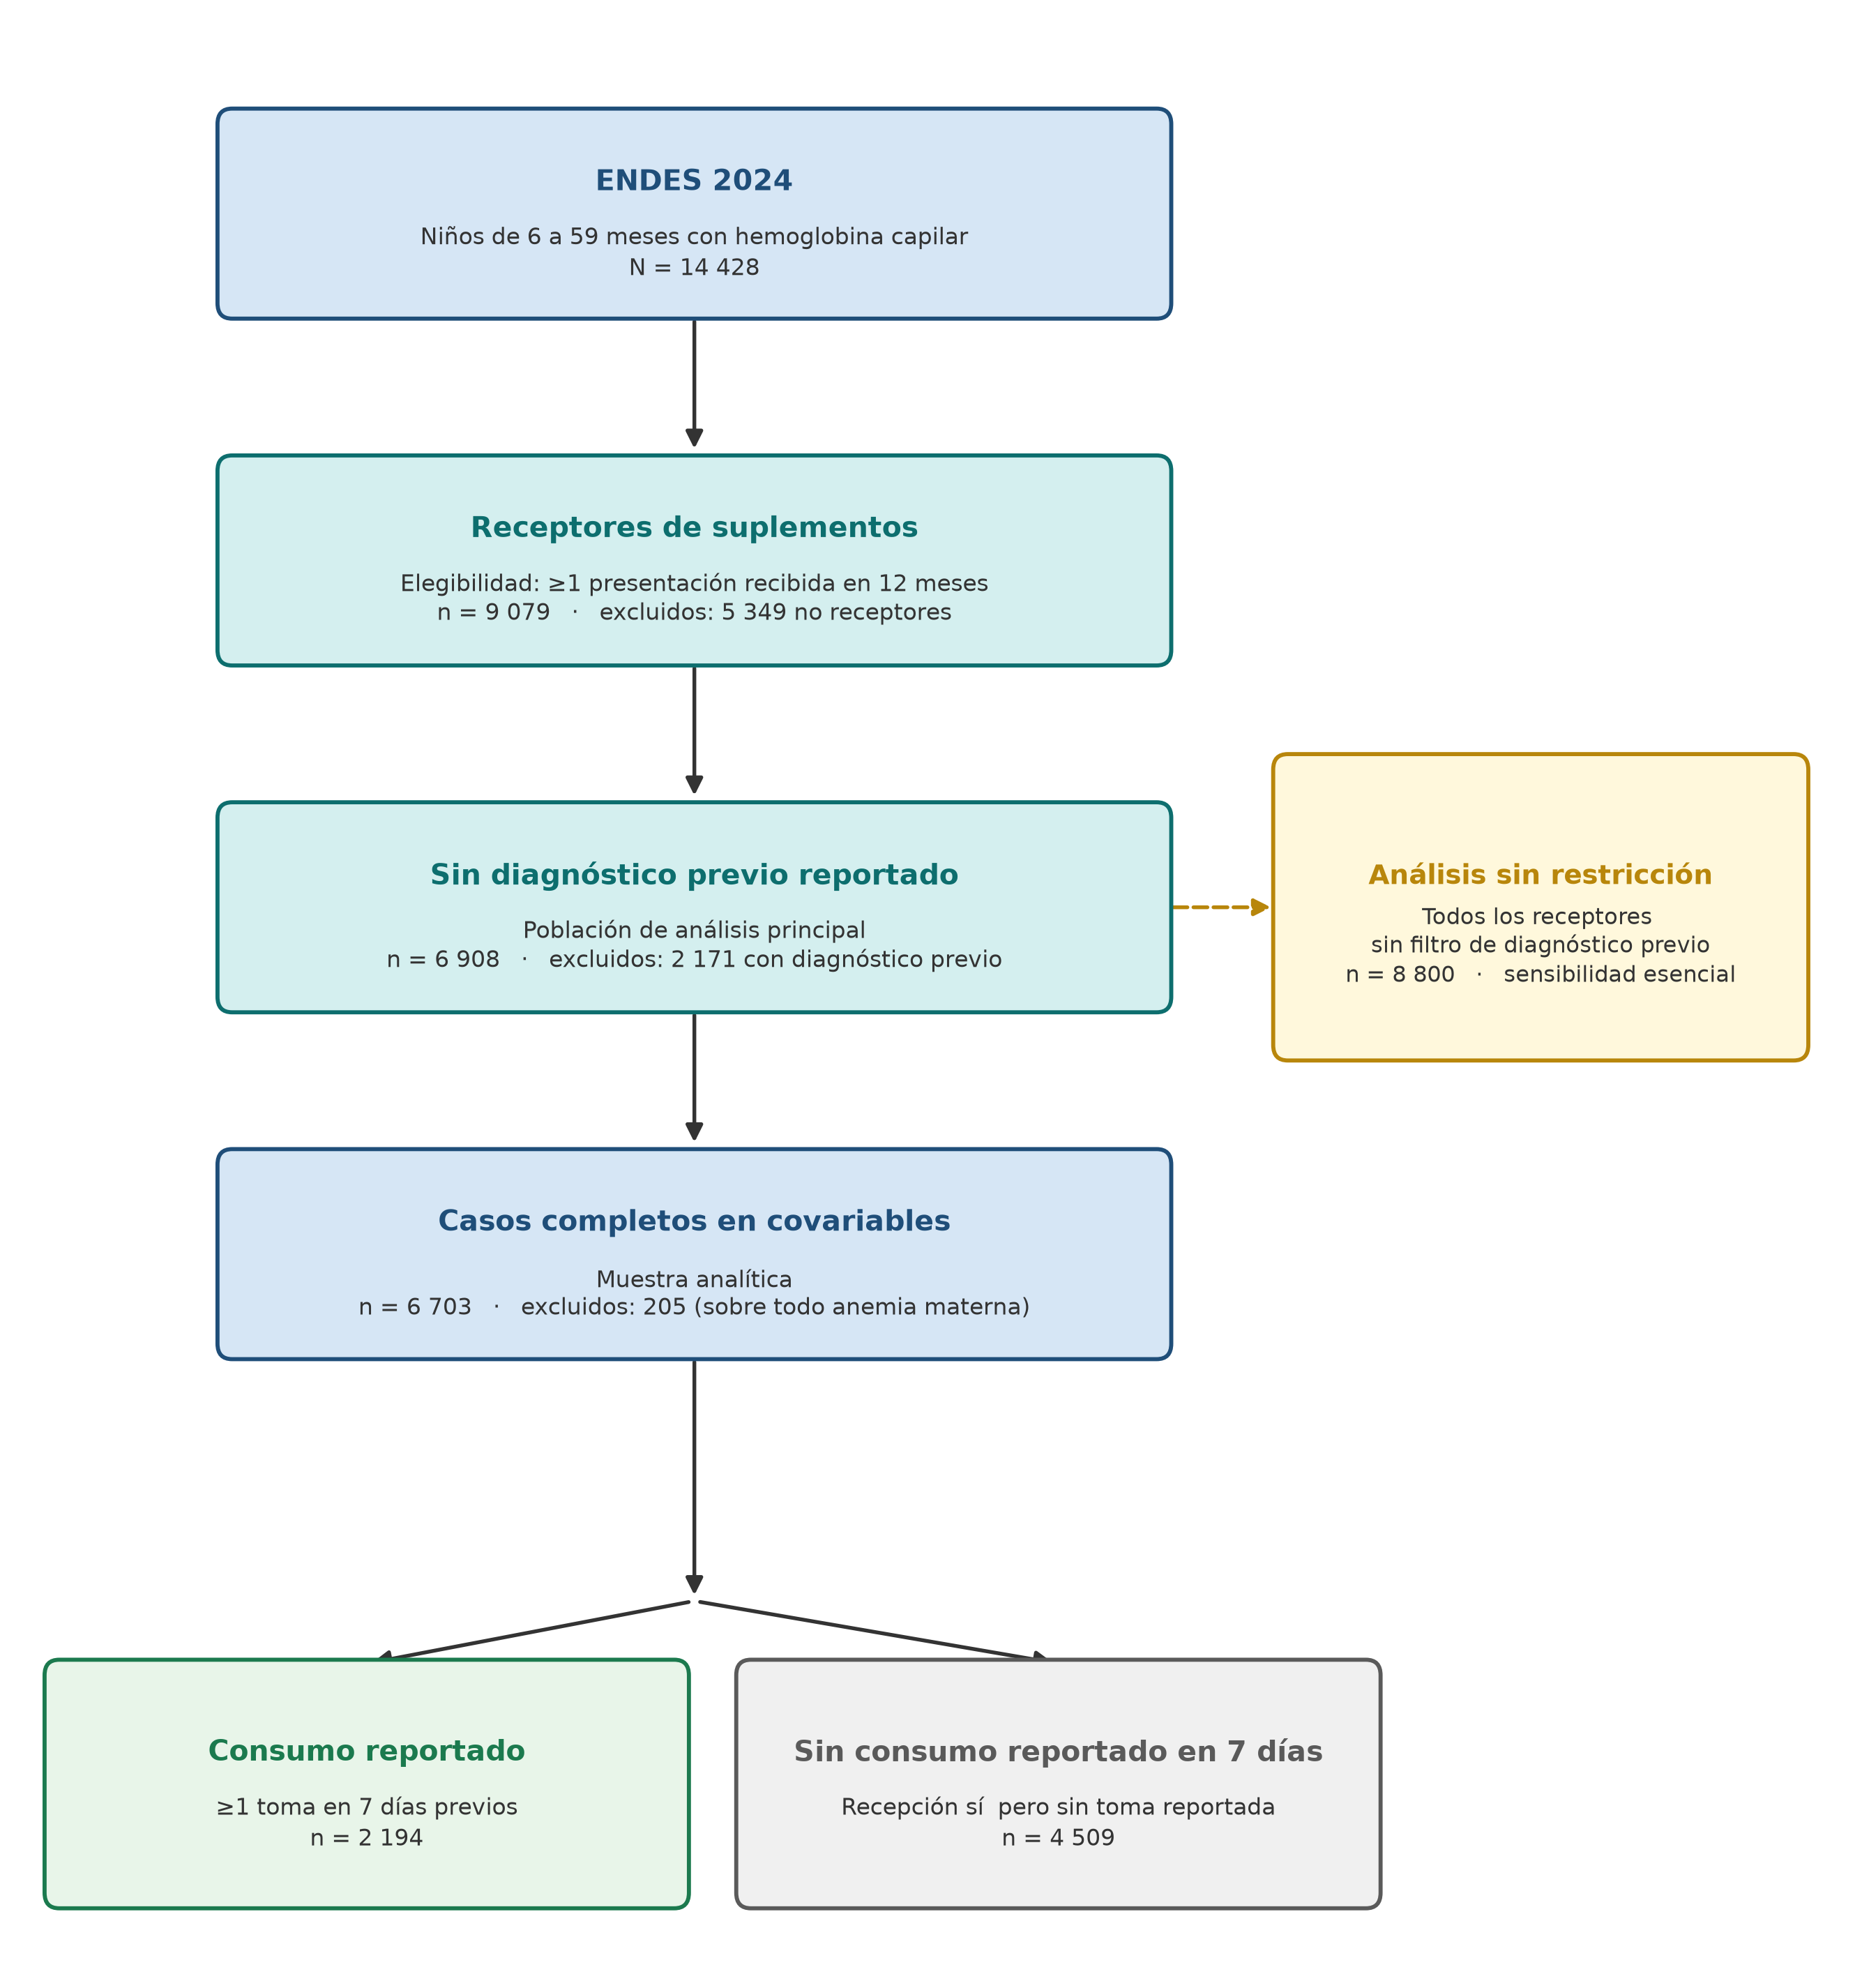
\includegraphics[width=.92\linewidth]{figura_flujo_muestral.png}
	\caption{Flujo de selección desde la ENDES 2024 hasta la muestra analítica. La rama lateral resume el análisis sin restricción por diagnóstico previo, reportado en Resultados como sensibilidad esencial.}
	\label{fig:flujo}
\end{figure}

Dado que la ENDES es de diseño transversal, la exposición se reporta retrospectivamente y el desenlace se mide en la misma visita; por tanto, no es posible verificar el orden temporal entre el consumo y la anemia, lo que condiciona toda interpretación posterior.


\subsection{Variables}

Se definió la exposición como el consumo reportado de al menos una de las cuatro presentaciones de hierro (jarabe, gotas, polvos de micronutrientes u otro) durante los siete días previos a la encuesta (preguntas \texttt{s465ea}--\texttt{s465ed}). La elegibilidad exigía haber recibido el suplemento en algún momento de los 12 meses anteriores. Cabe precisar que una sola toma reportada basta para clasificar al niño como expuesto: el dato de la ENDES no permite medir dosis exacta, frecuencia ni adherencia real, y la etiqueta de ``suplemento de hierro'' se toma del cuestionario sin verificar su composición química.

El desenlace principal fue la anemia moderada o severa según los umbrales del MINSA. Se priorizó este nivel de severidad por su mayor impacto en el desarrollo infantil y en la carga de los servicios de salud. Los desenlaces secundarios fueron: anemia de cualquier grado; hemoglobina MINSA y OMS (g/L); e índice ordinal de severidad derivado de \texttt{niveles\_anemia} (0 = sin anemia, 1 = leve, 2 = moderada/severa). Para la multiplicidad de estos cuatro secundarios se aplicó la corrección de Holm--Bonferroni sobre los valores $p$ del estimador IPW$\times$diseño (errores HC3), dejando el primario fuera de la familia de contraste. Se consideró un valor de $p<0{,}05$ como estadísticamente significativo. Para facilitar la interpretación clínica, la hemoglobina se reportó en g/L; para la conversión de unidades, $1$ g/dL equivale a $10$ g/L.


Como covariables para el puntaje de propensión se incluyeron edad del niño en forma polinómica, sexo, bajo peso al nacer, edad y educación maternas, anemia materna, control prenatal, quintil de riqueza, acceso a agua, saneamiento y área urbana. Se excluyó deliberadamente la diarrea reciente porque su ventana de medición no permite establecer que precediera al consumo y podría ser consecuencia de este o compartir causas con la anemia. Dada la naturaleza transversal de la ENDES, se asumió que las covariables incluidas representan condiciones previas o simultáneas al consumo, aunque no es posible verificar su antecedencia temporal estricta.

Se trataron los casos con datos faltantes en el consumo (18--22 niños en la base total, según el componente) como ausencia de toma en el análisis principal, para mantener la consistencia con la codificación del microdato. Se realizó un análisis de sensibilidad excluyéndolos y los resultados no variaron, por lo que se mantuvo la muestra original de 6\,703 casos.

\begin{table}[htbp]
	\centering
	\caption{Definición operacional de exposición, desenlaces y covariables}
	\label{tab:ops}
	\small
	\begingroup
	\renewcommand{\arraystretch}{1.15}
	\setlength{\tabcolsep}{6.9pt}
	\setlength{\heavyrulewidth}{0.75pt}
	\setlength{\lightrulewidth}{0.5pt}
	\begin{tabular}{p{3.1cm}p{12.2cm}}
		\toprule
		Elemento               & Definición                                                                                                                                                                                                                                                                                                                                                                                  \\
		\noalign{\setlength{\lightrulewidth}{0.75pt}}
		\midrule
		\noalign{\setlength{\lightrulewidth}{0.5pt}}
		Población              & Niños de 6--59 meses con hemoglobina en ENDES 2024 que recibieron $\ge$1 presentación de suplemento (12 meses). Análisis principal: sin diagnóstico previo de anemia reportado por la madre.                                                                                                                                                                                                \\
		Exposición             & Consumo reportado de al menos una presentación del módulo de hierro en los 7 días previos (\texttt{toma7d\_jar/got/pol/otr}; ENDES \texttt{s465ea}, \texttt{s465ec}, \texttt{s465eb}, \texttt{s465ed}) frente a recepción sin ese consumo. No es dosis ni adherencia. Faltantes de toma: 18--22 en el archivo completo (2 en la muestra analítica); el principal los trata como no consumo. \\
		Elegibilidad           & Recepción en 12 meses: \texttt{rec12m\_*} (\texttt{s465db\_a}--\texttt{d}). Ventana distinta de la exposición.                                                                                                                                                                                                                                                                              \\
		Desenlace principal    & Anemia moderada o severa (criterio MINSA; HemoCue ajustada por altitud).                                                                                                                                                                                                                                                                                                                    \\
		Desenlaces secundarios & Anemia de cualquier grado; Hb MINSA y OMS (g/L); índice ordinal de severidad.                                                                                                                                                                                                                                                                                                               \\
		Covariables            & Edad (cúbica), sexo, bajo peso al nacer, edad y educación materna, anemia materna, control prenatal, quintil, agua, saneamiento, área. Departamento solo en el modelo complementario.                                                                                                                                                                                                       \\
		Datos faltantes        & Casos completos ($n=6\,703$ de 6\,908). Sensibilidad: reponderación por probabilidad de ser caso completo y exclusión de tomas faltantes.                                                                                                                                                                                                                                                                           \\
		\bottomrule
	\end{tabular}
	\endgroup
\end{table}

\subsection{Estimación}

El estimando principal fue la diferencia de prevalencias de anemia moderada o severa entre niños con y sin consumo reportado, estimada mediante ponderación por el inverso de la probabilidad de exposición combinada con el peso de diseño de la ENDES, en la muestra analítica de receptores sin diagnóstico previo reportado. Se calculó un puntaje de propensión logístico \emph{sin} pesos de encuesta en el análisis principal; la ponderación por el inverso de la probabilidad de exposición (IPW) se estabilizó por la prevalencia observada y se multiplicó después por el peso de diseño de la ENDES ($w_{\text{diseño}}=\texttt{hv005}/10^6$, renormalizado a media 1). Para la inferencia se utilizó remuestreo bootstrap estratificado con 2\,000 réplicas, respetando los conglomerados (\texttt{hv001}) dentro de cada estrato (\texttt{hv022}; 240 estratos en la base). En cada réplica se reestimó el puntaje de propensión, se recalcularon los pesos IPW y el peso de diseño renormalizado, y se volvió a estimar la diferencia de prevalencias. La base ENDES utilizada contiene 3\,193 valores únicos de conglomerado (\texttt{hv001}) en el archivo analítico completo. No se contaba con las variables \texttt{hv021} ni \texttt{hv023} del diseño muestral original, por lo que la estructura de varianza se basó en \texttt{hv001} y \texttt{hv022}. Se reportó el intervalo percentil bootstrap como medida principal de incertidumbre.

El modelo de referencia no incluyó el departamento. En un análisis complementario se incorporó al modelo del puntaje de propensión como proxy de heterogeneidad territorial y se consideró una especificación conservadora, dado que se esperaba una atenuación de la asociación si existían diferencias estructurales entre regiones. En el cuerpo del artículo se reportan también el análisis sin filtro de diagnóstico previo, la definición alternativa de consumo en 12 meses (cantidades \texttt{qtoma12m\_*}) y la reponderación por probabilidad de ser caso completo. Los estimadores alternativos ---emparejamiento y doble robustez--- se presentan en el material suplementario y no se interpretan como réplicas del análisis principal, porque responden a supuestos distintos.

\subsection{Ética y reproducibilidad}

Este estudio utilizó exclusivamente microdatos secundarios públicos y anonimizados de la ENDES 2024, sin intervención, contacto con participantes ni recolección de datos nuevos. Los microdatos se obtuvieron bajo las condiciones de acceso público del INEI y se manejan conforme a la normativa peruana de protección de datos personales (Ley~29733). En el repositorio del proyecto no consta una determinación formal de exención emitida por un comité de ética institucional; por ello no se atribuye aquí un nombre de comité ni un número de aprobación. Se fijó la semilla 20260710 para favorecer la reproducibilidad de los resultados. El análisis se ejecutó con Python 3.11.15 y las versiones congeladas de las bibliotecas de cómputo registradas en el archivo de bloqueo del repositorio (\texttt{requirements-lock.txt}): pandas 3.0.5, NumPy 2.4.6, SciPy 1.15.3, statsmodels 0.14.6, scikit-learn 1.9.0 y Matplotlib 3.11.1, en un entorno conda sobre macOS (Apple Silicon). El PDF del manuscrito se generó con pdfLaTeX y Biber (TeX Live 2025).

%==============================================================================
\section{RESULTADOS}
%==============================================================================

\subsection{Muestra y balance}

En la muestra analítica, la prevalencia cruda de anemia fue 37{,}9\%. Los niños con consumo reportado fueron considerablemente más jóvenes (media 19{,}9 frente a 29{,}7 meses) y presentaron un perfil hematológico desfavorable: 44{,}9\% de anemia de cualquier grado frente a 34{,}5\% (986 frente a 1\,555 casos de cualquier grado), 14{,}9\% de anemia moderada o severa frente a 9{,}9\% (327 frente a 447 eventos), y una hemoglobina MINSA 2{,}6 g/L menor en promedio (110{,}4 frente a 113{,}0 g/L; tabla~\ref{tab:desc}). Este desequilibrio basal fue compatible con diferencias sistemáticas entre los grupos, potencialmente relacionadas con confusión por indicación. La ponderación se utilizó para reducir el desequilibrio de las covariables observadas.

\begin{table}[htbp]
	\centering
	\caption{Características según consumo reportado y balance posponderación}
	\label{tab:desc}
	\begingroup
	\renewcommand{\arraystretch}{1.15}
	\setlength{\tabcolsep}{6.9pt}
	\setlength{\heavyrulewidth}{0.75pt}
	\setlength{\lightrulewidth}{0.5pt}
	\resizebox{\linewidth}{!}{%
		\begin{tabular}{lcccc}
			\toprule
			Variable                             & Consumo ($n=2\,194$) & Sin consumo ($n=4\,509$) & Total ($n=6\,703$) & $|$DME$|$ post-IPW \\
			\noalign{\setlength{\lightrulewidth}{0.75pt}}
			\midrule
			\noalign{\setlength{\lightrulewidth}{0.5pt}}
			Edad niño (meses), media (DE)        & 19{,}9 (13{,}0)      & 29{,}7 (14{,}2)          & 26{,}5 (14{,}6)    & 0{,}021            \\
			Edad$^{2}$ (centrada)                & ---                  & ---                      & ---                & 0{,}023            \\
			Edad$^{3}$ (centrada)                & ---                  & ---                      & ---                & 0{,}039            \\
			Sexo femenino, \%                    & 49{,}6               & 49{,}8                   & 49{,}7             & 0{,}007            \\
			Bajo peso al nacer, \%               & 6{,}3                & 6{,}5                    & 6{,}5              & 0{,}013            \\
			Edad materna (años), media (DE)      & 29{,}9 (7{,}1)       & 30{,}6 (6{,}9)           & 30{,}4 (7{,}0)     & 0{,}012            \\
			Educación materna (0--3), media (DE) & 2{,}2 (0{,}7)        & 2{,}2 (0{,}7)            & 2{,}2 (0{,}7)      & 0{,}000            \\
			Anemia materna, \%                   & 25{,}7               & 24{,}0                   & 24{,}5             & 0{,}007            \\
			Control prenatal, \%                 & 94{,}4               & 92{,}0                   & 92{,}8             & 0{,}001            \\
			Quintil de riqueza, media (DE)       & 2{,}3 (1{,}2)        & 2{,}3 (1{,}2)            & 2{,}3 (1{,}2)      & 0{,}019            \\
			Agua potable, \%                     & 72{,}7               & 71{,}8                   & 72{,}1             & 0{,}009            \\
			Saneamiento, \%                      & 60{,}3               & 60{,}9                   & 60{,}7             & 0{,}006            \\
			Área urbana, \%                      & 64{,}7               & 64{,}9                   & 64{,}8             & 0{,}010            \\
			\midrule
			Anemia de cualquier grado, \%        & 44{,}9               & 34{,}5                   & 37{,}9             & ---                \\
			Anemia moderada o severa, \%         & 14{,}9               & 9{,}9                    & 11{,}5             & ---                \\
			Hb MINSA (g/L), media (DE)           & 110{,}4 (10{,}8)     & 113{,}0 (10{,}4)         & 112{,}1 (10{,}6)   & ---                \\
			\bottomrule
		\end{tabular}%
	}
	\endgroup
\end{table}

Tras la ponderación IPW, el balance fue aceptable: ninguna covariable superó 0{,}10 en diferencia de medias estandarizada y el máximo absoluto fue 0{,}039. Los pesos fueron moderados, con un percentil 99 de 2{,}81 y un máximo de 6{,}55. Solo 12 observaciones (0{,}18\%) quedaron fuera del rango de solapamiento $[0{,}05;\,0{,}95]$ (figura~\ref{fig:love}), lo que indicó una pérdida de solapamiento pequeña pero presente.

\begin{figure}[htbp]
	\centering
	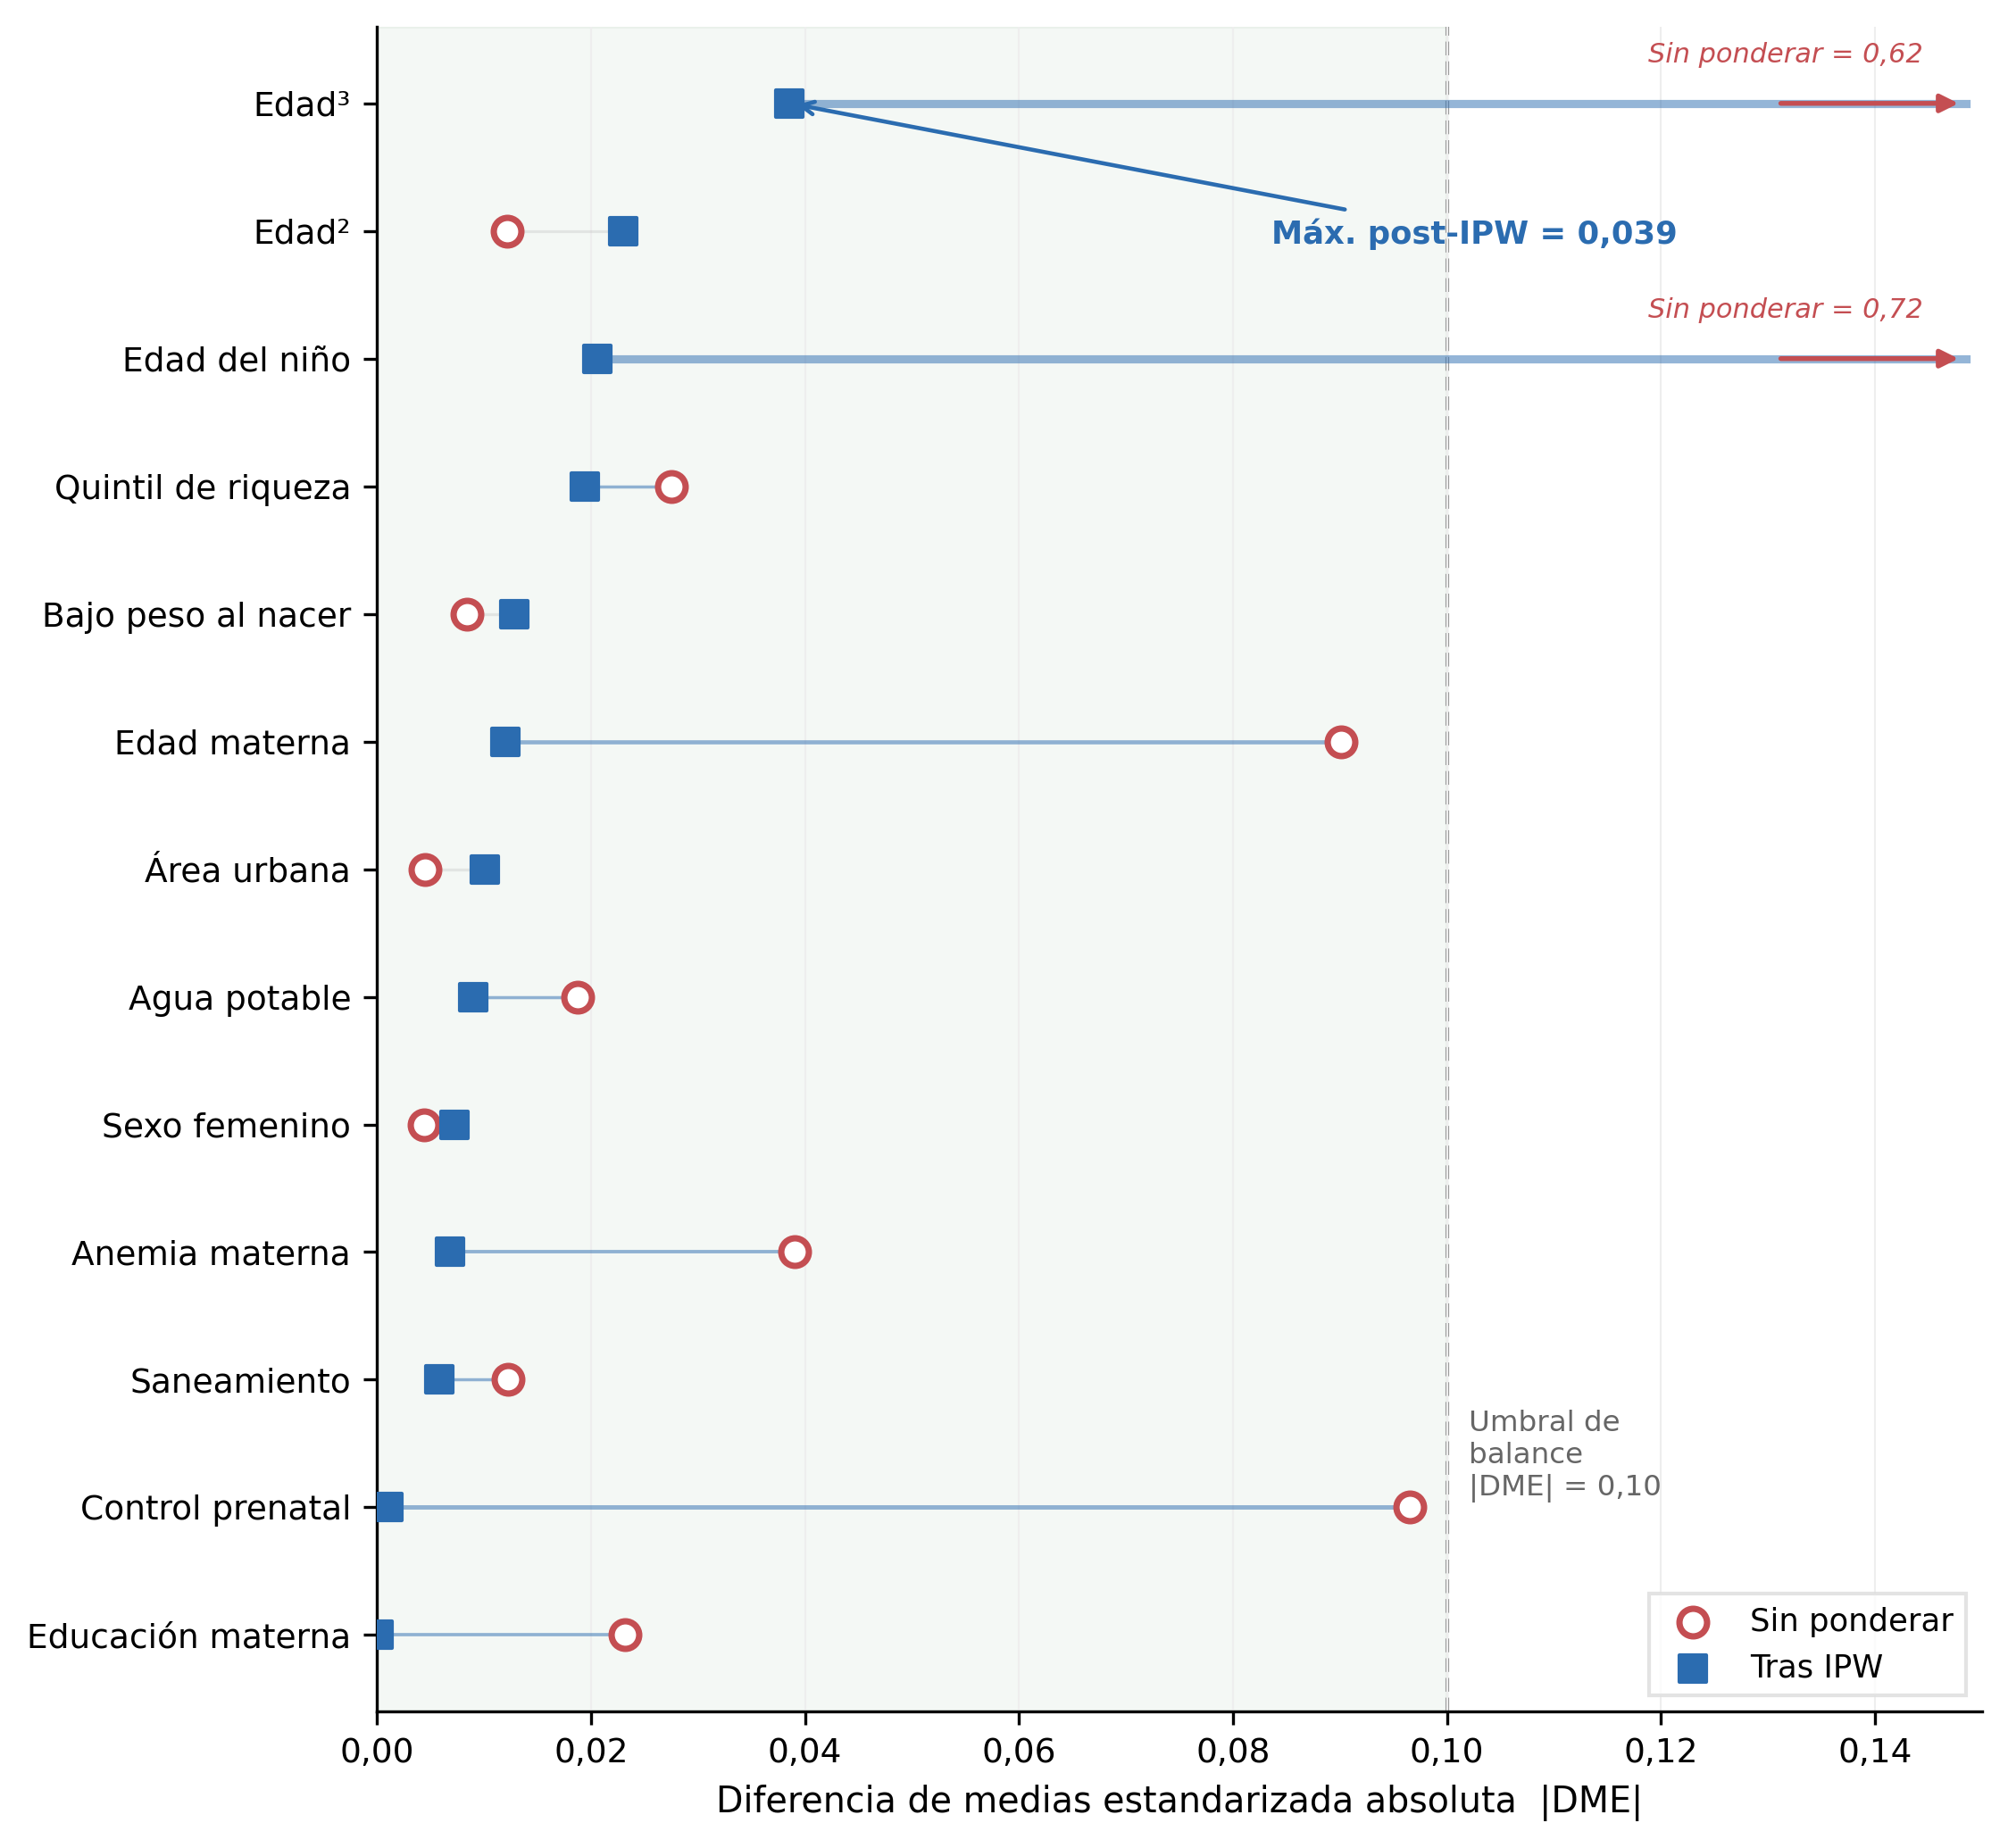
\includegraphics[width=.92\linewidth]{figura_1_love_plot.png}
	\caption{Balance de covariables antes y después de la ponderación IPW. Todas las diferencias de medias estandarizadas absolutas posponderación permanecen por debajo de 0{,}10.}
	\label{fig:love}
\end{figure}

\subsection{Asociación principal y sensibilidades esenciales}

Según el estimador de referencia ---IPW combinado con peso de diseño, sin departamento, sobre la muestra analítica de receptores sin diagnóstico previo reportado---, las prevalencias ajustadas de anemia moderada o severa fueron 9{,}3\% entre consumidores y 12{,}1\% entre no consumidores: una diferencia de $-2{,}8$ puntos porcentuales (IC del 95\% bootstrap $[-4{,}5;\,-1{,}2]$; 327 frente a 447 eventos) (tabla~\ref{tab:main}; figura~\ref{fig:bosque}). Al añadir el departamento al modelo, la estimación se atenuó a $-2{,}4$ puntos porcentuales (IC del 95\% $[-4{,}1;\,-0{,}7]$). En el análisis sin filtro de diagnóstico previo, restringido a casos completos ($n=8\,800$; 3\,110 con consumo), la diferencia cayó a $-0{,}9$ puntos porcentuales e incluyó el nulo (IC del 95\% $[-2{,}6;\,0{,}9]$). Con la definición alternativa de consumo en 12 meses, la estimación puntual cambió de signo ($+2{,}4$ puntos porcentuales), pero su intervalo de confianza fue compatible con el nulo (IC del 95\% $[-0{,}2;\,4{,}7]$); en esa especificación 5\,992 de los 6\,703 niños (89{,}4\%) figuraban como expuestos y solo 711 como controles, de modo que la positividad fue limitada y el contraste fue apenas identificable.

\begin{table}[htbp]
	\centering
	\caption{Estimaciones de asociación entre consumo reportado y anemia o hemoglobina}
	\label{tab:main}
	\resizebox{\linewidth}{!}{%
		\begin{tabular}{lccccc}
			\toprule
			Especificación                                                 & $n$ ($n$ consumo) & Estimación & IC del 95\% & $p$ & $p$ ajustado \\                                                                                                                                                                                                                                                                                              \\
			\midrule
			Anemia moderada o severa, IPW$\times$diseño\textsuperscript{a} & 6\,703 (2\,194)   & $-2{,}8$ & $[-4{,}5;\,-1{,}2]$ & --- & ---                                                                                                                                                                                                                                                                                  \\
			Con ajuste departamental                                       & 6\,703 (2\,194)   & $-2{,}4$ & $[-4{,}1;\,-0{,}7]$ & --- & ---                                                                                                                                                                                                                                                                                  \\
			Sin filtro de diagnóstico, casos completos                     & 8\,800 (3\,110)   & $-0{,}9$ & $[-2{,}6;\,0{,}9]$ & --- & ---                                                                                                                                                                                                                                                                                   \\
			Consumo reportado en 12 meses                                  & 6\,703 (5\,992)   & $+2{,}4$ & $[-0{,}2;\,4{,}7]$ & --- & ---                                                                                                                                                                                                                                                                                   \\
			Anemia de cualquier grado\textsuperscript{b}                    & 6\,703 (2\,194)   & $-2{,}6$ & $[-5{,}0;\,0{,}4]$ & $0{,}117$ & $0{,}196$                                                                                                                                                                                                                                                                                   \\
			Índice ordinal de severidad\textsuperscript{b}                 & 6\,703 (2\,194)   & $-5{,}4$ & $[-8{,}8;\,-1{,}3]$ & $0{,}017$ & $0{,}066$                                                                                                                                                                                                                                                                                  \\
			Hb MINSA (g/L)\textsuperscript{b}                              & 6\,703 (2\,194)   & $+0{,}65$  & $[-0{,}04;\,1{,}24]$ & $0{,}075$ & $0{,}196$                                                                                                                                                                                                                                                                                     \\
			Hb OMS (g/L)\textsuperscript{b}                                & 6\,703 (2\,194)   & $+0{,}67$  & $[0{,}00;\,1{,}25]$ & $0{,}065$ & $0{,}196$                                                                                                                                                                                                                                                                                      \\
			\bottomrule
			\multicolumn{6}{p{17cm}}{\textsuperscript{a} Prevalencias ajustadas por IPW$\times$diseño: 9{,}3\% con consumo reportado y 12{,}1\% sin consumo. IC de las cuatro primeras filas: percentiles bootstrap con 2\,000 réplicas. \textsuperscript{b} Desenlaces secundarios: IC percentil bootstrap del estimador de referencia; $p$ del IPW$\times$diseño (HC3). Ningún desenlace secundario alcanzó $\alpha{=}0{,}05$ tras la corrección de Holm--Bonferroni. Estimaciones en puntos porcentuales, excepto hemoglobina en g/L.} \\
		\end{tabular}%
	}
\end{table}

\begin{figure}[htbp]
	\centering
	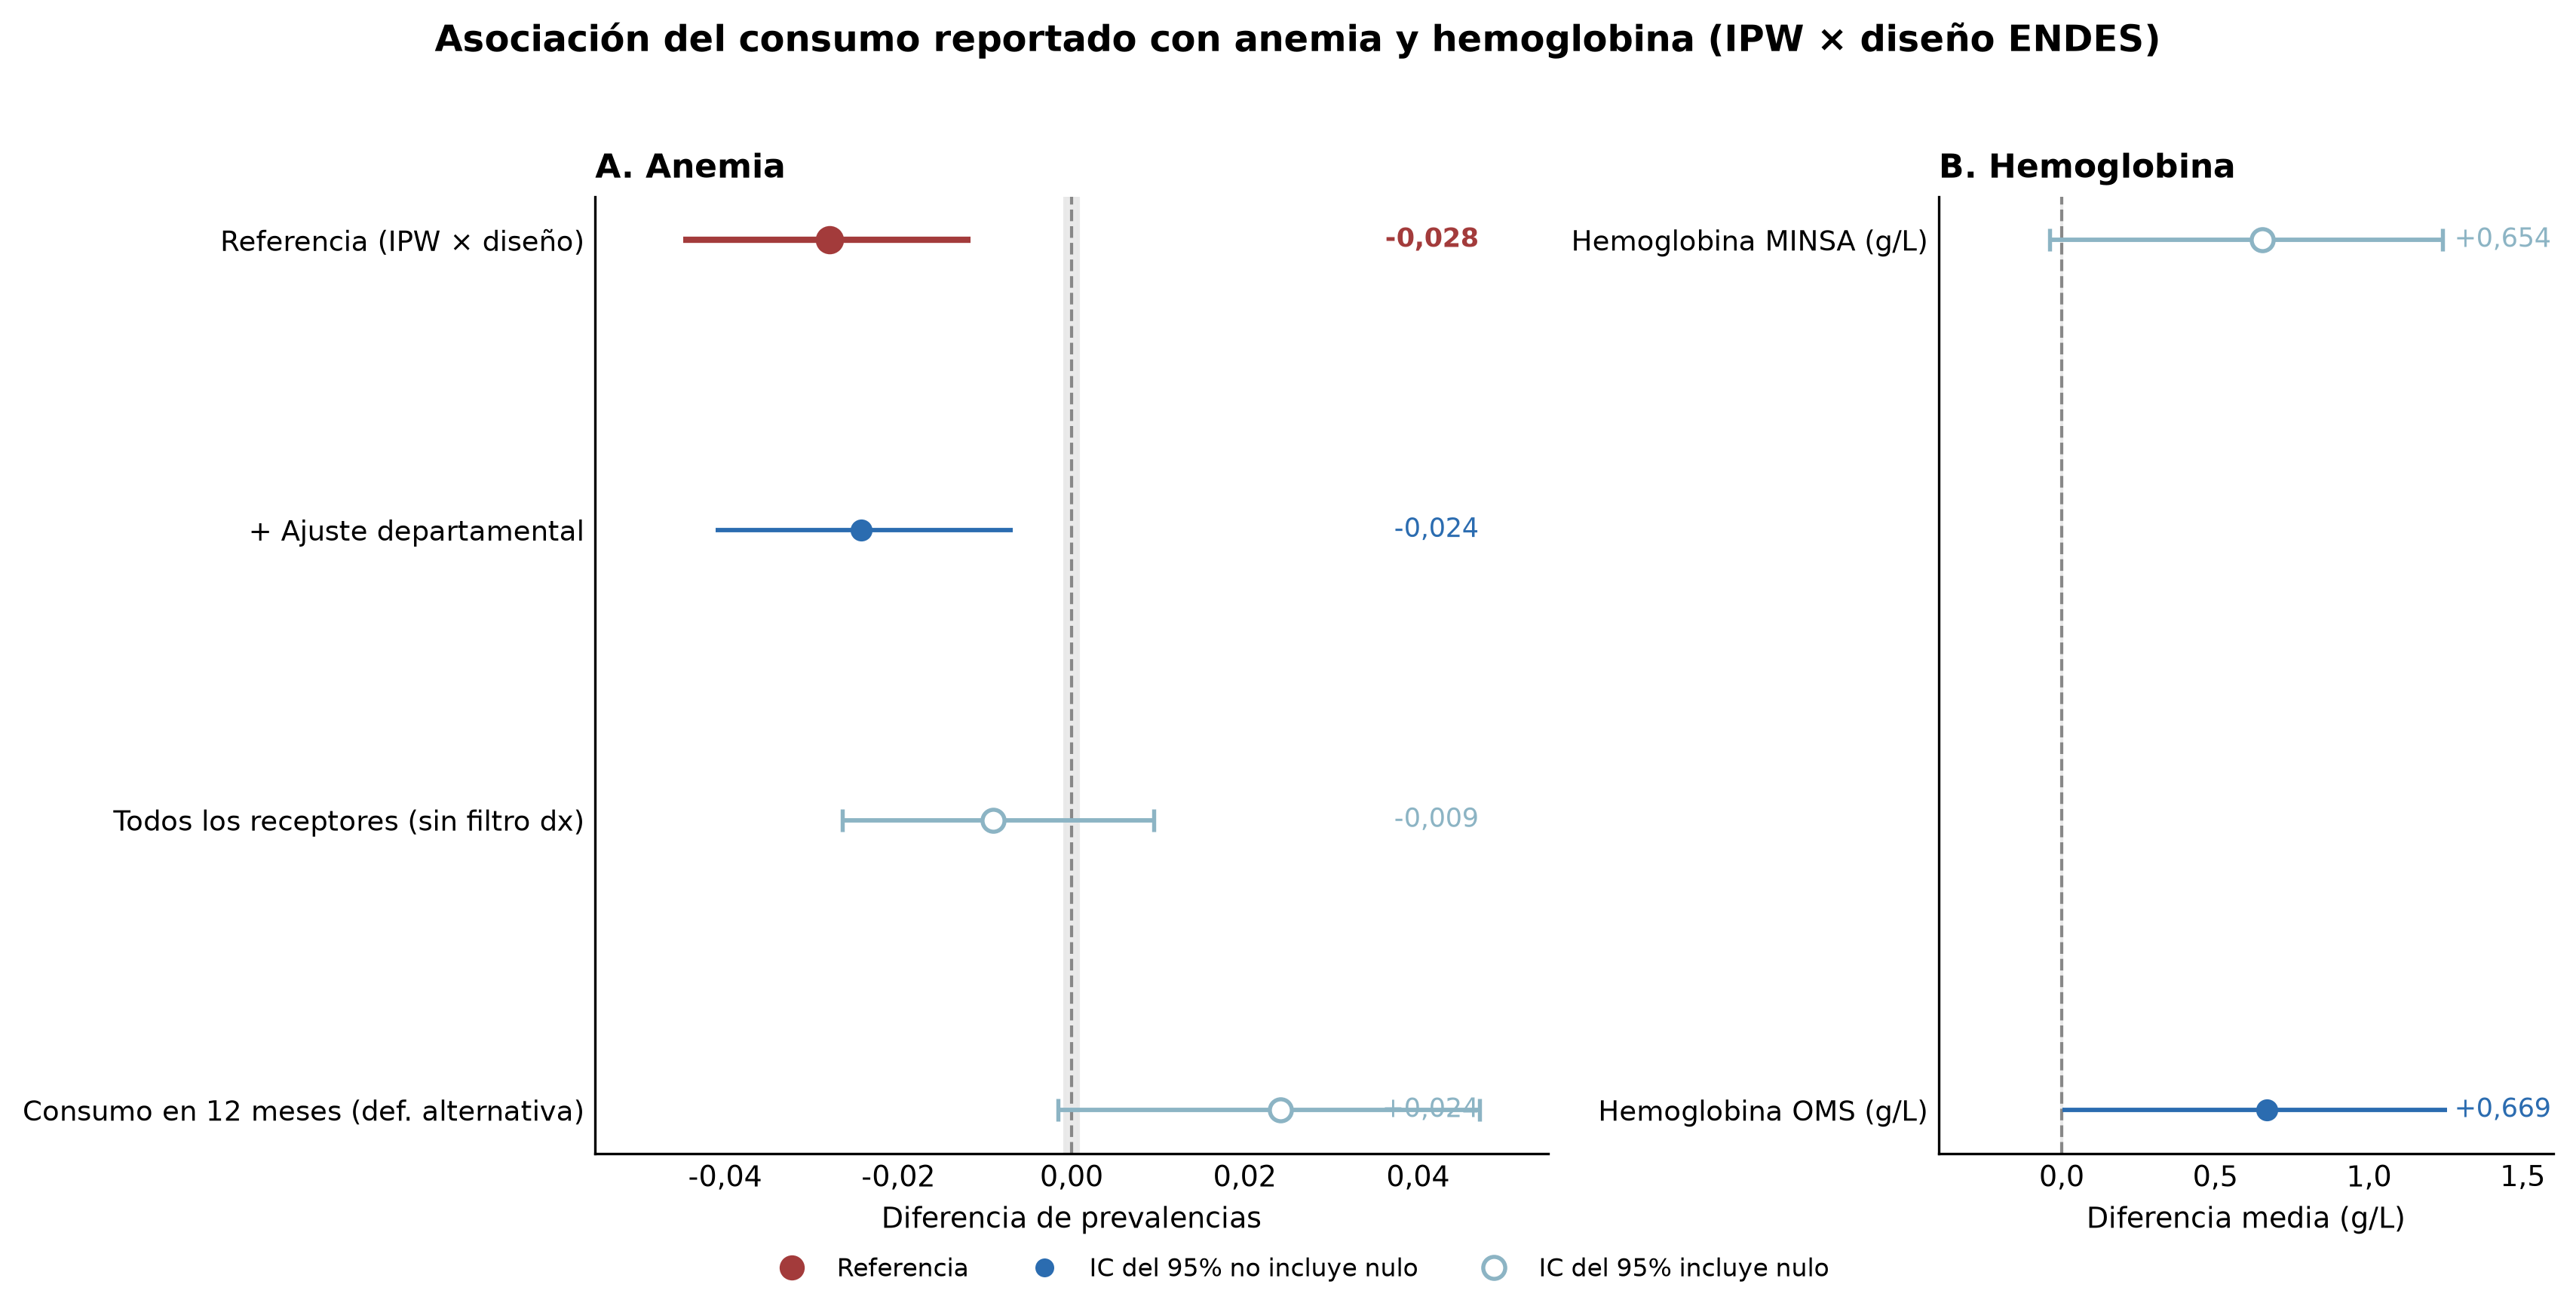
\includegraphics[width=.92\linewidth]{figura_bosque_esencial.png}
	\caption{Asociación del consumo reportado con anemia moderada o severa y hemoglobina. Los intervalos son percentil bootstrap del 95\%.}
	\label{fig:bosque}
\end{figure}

De los 6\,908 receptores sin diagnóstico previo, se perdieron 205 (3\%) al pasar a casos completos, prácticamente todos por anemia materna faltante. En la base total, la anemia materna presentó 449 observaciones faltantes; la educación materna y la edad materna presentaron pérdidas marginales inferiores al 0{,}1\% (tabla~\ref{tab:faltantes}). Las observaciones fuera del rango de solapamiento $[0{,}05;\,0{,}95]$ no fueron eliminadas ni se recortaron pesos en el estimador principal: se conservaron con su peso completo y las 12 observaciones (0{,}18\%) fuera de rango se reportaron como diagnóstico de positividad; un análisis de sensibilidad con recorte armonizó las estimaciones. La reponderación por probabilidad de ser caso completo no modificó el punto estimado: se mantuvo en $-2{,}8$ puntos porcentuales. La exclusión de los dos niños con toma faltante en la muestra analítica tampoco modificó la estimación.

El cociente de las prevalencias ajustadas, utilizado como aproximación al RR para el cálculo del E-value, fue $0{,}093/0{,}121 \approx 0{,}77$. Con la fórmula de VanderWeele y Ding para una asociación inversa, $E = 1/RR + \sqrt{(1/RR)\,(1/RR-1)}$, el E-value del punto fue $\approx 1{,}93$. Para el límite del intervalo más cercano al nulo ($-1{,}2$ puntos porcentuales), el cociente implícito fue $\approx 0{,}90$ y el E-value correspondiente fue $\approx 1{,}46$. Estos valores describen la sensibilidad de la asociación observada a una posible confusión no medida y no constituyen una prueba de causalidad \parencite{vanderweele2017}.


\subsection{Hemoglobina y desenlaces secundarios}

La diferencia media de hemoglobina MINSA fue pequeña: $+0{,}65$ g/L ($+0{,}065$ g/dL; IC del 95\% $[-0{,}04;\,1{,}24]$). El intervalo de confianza incluyó la ausencia de diferencia y no se observó un desplazamiento claro de la distribución hematológica.

Los desenlaces secundarios ---anemia de cualquier grado, índice ordinal de severidad y hemoglobina MINSA y OMS--- mostraron estimaciones en dirección compatible con el desenlace principal. El índice ordinal mostró una diferencia de $-5{,}4$ puntos porcentuales (IC del 95\% $[-8{,}8;\,-1{,}3]$; $p{=}0{,}017$; Holm $p{=}0{,}066$). Tras aplicar la corrección de Holm--Bonferroni a los cuatro desenlaces secundarios, ninguno alcanzó $\alpha{=}0{,}05$ (tabla~\ref{tab:main}). Aunque las estimaciones fueron concordantes en dirección, la evidencia no permitió establecer una asociación estable para los desenlaces secundarios.

%==============================================================================
\section{DISCUSIÓN}
%==============================================================================

La asociación principal fue modesta y mostró sensibilidad a las especificaciones analizadas: la estimación se atenuó después de incorporar el departamento al modelo y fue compatible con el nulo al ampliar la población. Con la definición alternativa de consumo en 12 meses, la estimación puntual cambió de signo, pero su intervalo de confianza fue compatible con el nulo. Las ventanas de recuerdo de 7 días y de 12 meses no capturan necesariamente el mismo fenómeno; por ello, el cambio de signo de la estimación puntual sugiere dependencia de la operacionalización de la exposición, sin demostrar por sí solo un mecanismo biológico. Dado el diseño transversal, la temporalidad incierta y la posibilidad de confusión residual, estos resultados no deben interpretarse como evidencia de una relación causal.

%%

La diferencia media de hemoglobina fue pequeña y su intervalo de confianza incluyó la ausencia de diferencia ($+0{,}65$ g/L, $+0{,}065$ g/dL). Las estimaciones de los desenlaces secundarios fueron imprecisas en varios casos y, tras aplicar la corrección de Holm--Bonferroni, ninguna alcanzó $\alpha{=}0{,}05$. En consecuencia, no se observó un desplazamiento claro de la distribución hematológica ni evidencia suficiente de una asociación estable entre el consumo reportado y los desenlaces secundarios.


%%

Los ensayos clínicos con adherencia supervisada ofrecen un referente de eficacia biológica que no puede trasladarse directamente a las condiciones de un programa de campo \parencite{low2013,who2016iron,neuberger2016}. En el Perú, las evaluaciones de proceso han documentado que la cobertura de entrega no garantiza el consumo ni la administración correcta \parencite{munares2018,minsa2022}. En este contexto, la asociación observada aporta información sobre la relación entre consumo reportado y estado hematológico, pero no permite determinar si la brecha entre entrega y consumo explica dicha asociación ni establecer cuánto de la asociación observada podría corresponder a la administración domiciliaria frente al error de medición o la confusión residual. Por tanto, el estudio examina un eslabón intermedio del funcionamiento programático, pero no constituye una prueba de eficacia del hierro en el hogar.


%%
El estudio tiene limitaciones que condicionan la interpretación de sus resultados. En primer lugar, el diseño transversal impide establecer temporalidad: la ENDES no registra si el consumo precedió a la anemia, las ventanas de recuerdo son distintas para elegibilidad (12 meses) y exposición (7 días), y una sola toma reportada basta para clasificar la exposición sin información de dosis, frecuencia ni adherencia. El consumo es autorreportado por la madre y puede verse afectado por sesgo de memoria, deseabilidad social y mala clasificación de la exposición. En segundo lugar, la selección de la población es vulnerable: excluir a niños con diagnóstico previo reportado puede sesgar la muestra ---``sin diagnóstico reportado'' no equivale a ``sin anemia previa''--- y el hallazgo depende de esa decisión. La recepción o el consumo reportados no permiten verificar que el producto proviniera exclusivamente del programa público. En tercer lugar, la medición es limitada: la hemoglobina detecta anemia, pero no identifica déficit de hierro; sin ferritina ni marcadores de inflamación no es posible atribuir la anemia observada a ferropenia. Tratar tomas faltantes como ausencia de consumo, aunque se evaluó mediante un análisis de sensibilidad, puede introducir mala clasificación si los faltantes no son aleatorios. Además, faltan variables como dieta, parasitosis o contacto sanitario detallado, y el E-value del punto ($\approx 1{,}93$; límite del IC $\approx 1{,}46$) indica que una confusión no medida de magnitud moderada podría explicar la estimación puntual. Finalmente, la inferencia se basó en una aproximación parcial del diseño muestral, porque se utilizaron \texttt{hv001} y \texttt{hv022} en ausencia de \texttt{hv021} y \texttt{hv023}; además, los datos corresponden a un solo año.



Entre las fortalezas se encuentran la medición de la hemoglobina mediante HemoCue con ajuste por altitud, la restricción del análisis a quienes reportaron recepción de suplementos, el balance posponderación aceptable y la presentación explícita de sensibilidades que atenuaron la asociación o la hicieron compatible con el nulo. El análisis de omisión secuencial mostró que la edad del niño fue la covariable con mayor influencia: al omitirla, el signo de la estimación puntual se invirtió. Esta inversión indica que la dirección de la asociación depende sustancialmente del ajuste por edad y de su forma funcional, lo que refuerza la interpretación cautelosa del resultado principal. No demuestra que el ajuste haya eliminado toda la confusión residual.


En conclusión, en receptores de suplementos sin diagnóstico previo reportado, se observó una asociación modesta entre el consumo reportado durante los siete días anteriores y una prevalencia 2{,}8 puntos porcentuales menor de anemia moderada o severa. La estimación se atenuó después de incorporar el departamento al modelo, fue compatible con el nulo al ampliar la población y, con la definición alternativa de consumo en 12 meses, la estimación puntual cambió de signo; su intervalo de confianza correspondiente también fue compatible con el nulo. En conjunto, la sensibilidad a la población y a la ventana de exposición, sumada al diseño transversal, impide interpretar el hallazgo como evidencia de eficacia farmacológica o relación causal. Se recomienda estandarizar la medición del consumo reportado mediante ventanas de recuerdo claramente definidas y complementarla con mediciones de hemoglobina en la misma población. Para evaluar si una mejora en el consumo modifica la anemia infantil, se requieren estudios longitudinales con tiempo cero clínico definido, biomarcadores de hierro y validación del autorreporte frente a registros directos.


%==============================================================================
\section*{MATERIAL SUPLEMENTARIO}
%==============================================================================

\subsection{S1. Definiciones y flujo}

La Figura~\ref{fig:flujo} resume la selección. Se definió recibir al menos una presentación como T1${}=1$, o $n_{\text{recibidos}}\ge 1$, o un total de unidades recibidas ${}>0$. La exposición del artículo correspondió al consumo de al menos una de las cuatro presentaciones durante los siete días previos (\texttt{toma7d\_*}). El índice T5 del microdato, dicotomizado en $\ge 1$, coincidió con esta definición en la muestra analítica; el valor 5 del índice no se utilizó. El diagnóstico previo correspondió a un autorreporte materno y no estuvo fechado respecto del consumo. Esta subsección incluye la tabla de datos faltantes. Los estimadores alternativos se presentan en la subsección S2.

\begin{table}[htbp]
\centering
\caption{Datos faltantes en variables clave de la base ENDES utilizada ($N=14\,428$)}
\label{tab:faltantes}
\small
\begin{tabular}{lrr}
\toprule
Variable & $n$ faltantes & \% \\
\midrule
Anemia materna (\texttt{madre\_anemia}) & 449 & 3{,}11 \\
Educación materna (\texttt{educa\_madre}) & 9 & 0{,}06 \\
Edad materna (\texttt{edad\_madre}) & 9 & 0{,}06 \\
\bottomrule
\multicolumn{3}{p{10cm}}{\footnotesize Otras covariables del modelo de propensión no presentaron datos faltantes en la base analizada.} \\
\end{tabular}
\end{table}

\subsection{S2. Pesos, positividad y especificaciones alternativas}

La IPW se estabilizó por la prevalencia de la exposición y se multiplicó por el peso de diseño renormalizado. El solapamiento fue amplio (12 observaciones con puntaje ${}<0{,}05$; ninguna ${}>0{,}95$). El recorte de pesos y la imputación múltiple se calcularon también como análisis de sensibilidad; sus estimaciones puntuales y intervalos fueron consistentes con los de la especificación principal. Los estimadores alternativos de emparejamiento 1:1 y doble robustez se aplicaron a la misma muestra analítica y al mismo desenlace principal, con los resultados de la tabla~\ref{tab:suplementaria_estimadores}; respondieron a supuestos distintos y no se interpretaron como réplicas del estimador principal.

\begin{table}[htbp]
    \centering
    \caption{Estimadores alternativos para la asociación entre consumo reportado y anemia moderada o severa}
    \label{tab:suplementaria_estimadores}
    \small
    \begingroup
    \renewcommand{\arraystretch}{1.15}
    \setlength{\heavyrulewidth}{0.75pt}
    \setlength{\lightrulewidth}{0.5pt}
    \begin{tabular}{lccc}
        \toprule
        Estimador & Estimación & IC del 95\,\% & Muestra analítica \\
        \noalign{\setlength{\lightrulewidth}{0.75pt}}
        \midrule
        \noalign{\setlength{\lightrulewidth}{0.5pt}}
        Emparejamiento 1:1 (ATT) & $-0{,}024$ & $[-0{,}048;\,0{,}000]^{\textsuperscript{a}}$ & 1\,333 pares  \\
        Doble robustez (AIPW) & $-0{,}020$ & $[-0{,}036;\,-0{,}004]^{\textsuperscript{b}}$ & 6\,703 (2\,194 expuestos)  \\
        \bottomrule
        \multicolumn{4}{p{14.5cm}}{\footnotesize \textsuperscript{a} Intervalo asintótico normal para las diferencias pareadas (no bootstrap). \textsuperscript{b} Intervalo asintótico normal (estimación $\pm 1{,}96$ EE). Ninguno de los dos estimadores incorpora el peso de diseño de la ENDES. Los detalles metodológicos se describen en el texto.} \\
    \end{tabular}
    \endgroup
\end{table}

Como análisis de sensibilidad, el emparejamiento 1:1 estimó una diferencia de prevalencias de $-0{,}024$ ($-2{,}4$ puntos porcentuales; IC del 95\,\%: $-0{,}048$ a $0{,}0002$), y el estimador doblemente robusto produjo $-0{,}020$ ($-2{,}0$ puntos porcentuales; IC del 95\,\%: $-0{,}036$ a $-0{,}004$). El emparejamiento se restringió a los expuestos emparejados, sin peso de diseño, y utilizó un control único sin reuso; por el caliper, solo 1\,333 de los 2\,194 expuestos quedaron en el análisis. El estimador doblemente robusto estimó la diferencia de prevalencias sobre toda la muestra mediante validación cruzada de 5 pliegues. Ambos se presentan como sensibilidades bajo supuestos adicionales y \textbf{no} como demostración de causalidad ni como réplicas del estimador principal.

\subsection{S3. E-value y análisis restrictivos}

El cociente de las prevalencias ajustadas del estimador IPW$\times$diseño ($0{,}093/0{,}121\approx 0{,}77$) se utilizó como aproximación al RR para el cálculo del E-value; no corresponde a un riesgo relativo longitudinal observado. Con la fórmula de VanderWeele y Ding, el E-value del punto fue $\approx 1{,}93$ y el del límite del IC más cercano al nulo ($-1{,}2$ puntos porcentuales) fue $\approx 1{,}46$. Estos valores se obtuvieron a partir del cociente de prevalencias ajustadas del estimador principal, que combina IPW y peso de diseño, y no a partir de una estimación basada únicamente en IPW sin peso de diseño. El análisis sin filtro de diagnóstico, el ajuste departamental y el consumo en 12 meses se presentan en la tabla~\ref{tab:main}.


\section*{DECLARACIONES}

\textbf{Financiamiento.} Estudio autofinanciado.

\textbf{Conflictos de intereses.} Los autores declaran no tener conflictos de intereses.

\textbf{Contribuciones de autoría.} Rolando Bruno Bernaola Muñoz: construcción y curación de la base de datos, y desarrollo de la propuesta causal inicial. Jaime Enrique Lincovil Curivil: desarrollo del diseño del análisis y de los procedimientos de estimación y simulación. Niels Pacheco-Barrios: desarrollo del análisis y evaluación de los aspectos médicos. César Daniel Reinoso Reinoso: ejecución del algoritmo de búsqueda, ejecución del análisis, organización del repositorio de análisis y elaboración del reporte de análisis. Todos los autores participaron en la revisión crítica del manuscrito, aprobaron la versión final y asumen responsabilidad por el contenido del trabajo. Todos los autores declararon cumplir los criterios de autoría recomendados por el ICMJE.

\textbf{Disponibilidad de datos.} Los microdatos de la ENDES 2024 son públicos y están disponibles en el portal del INEI (\url{https://proyectos.inei.gob.pe/endes/}). El código de análisis, los datos derivados y las instrucciones de reproducción se distribuyen en el repositorio público del proyecto (endes2024-suplementos-hierro-anemia-peru); el identificador DOI del repositorio se añadirá cuando esté disponible.

%==============================================================================
\section*{Referencias}
%==============================================================================
\printbibliography[heading=none]

\end{document}
